\chapter{Results \& Discussion}
\label{chap:results}

\noindent This chapter reports the outcomes of our Clinical RAG evaluation and discusses the key findings. We reiterate the study aims: to quantify how different embedding models and small LLMs affect end-to-end retrieval-augmented answering quality, speed, and safety on a clinical QA set.

\section{Experiment Overview}
\begin{itemize}
  \item Total experiments: 54 runs (9 embedding models \(\times\) 6 LLMs).
  \item Embeddings: ms-marco, multi-qa, mini-lm, biomedbert, mpnet-v2, e5-base, BioLORD, BioBERT, MedQuAD.
  \item LLMs: deepseek, qwen, llama, gemma, phi3, tinyllama.
  \item Per-run questions: 20; metrics include pass rate, average score (primary), search time, documents found; efficiency/safety include throughput (QPM), disclaimer and hallucination rates.
\end{itemize}

\section{Overall Performance}
Aggregate results across all 54 runs show:
\begin{itemize}
  \item Average pass rate: 89.6\%.
  \item Average score: 0.706.
  \item Average search time: 98.77s.
\end{itemize}

Best-performing configurations:
\begin{itemize}
  \item Highest overall score: BioBERT + phi3 (avg. score 0.770, 100\% pass rate).
  \item Fastest: e5-base + deepseek (avg. search time 53.28s, avg. score 0.640).
\end{itemize}

\section{Comparison Heatmap}
Figure~\ref{fig:heatmap_avg_score} provides a model-by-model comparison heatmap (average score). An interactive version is available as HTML in the results folder.

\begin{figure}[h]
  \centering
  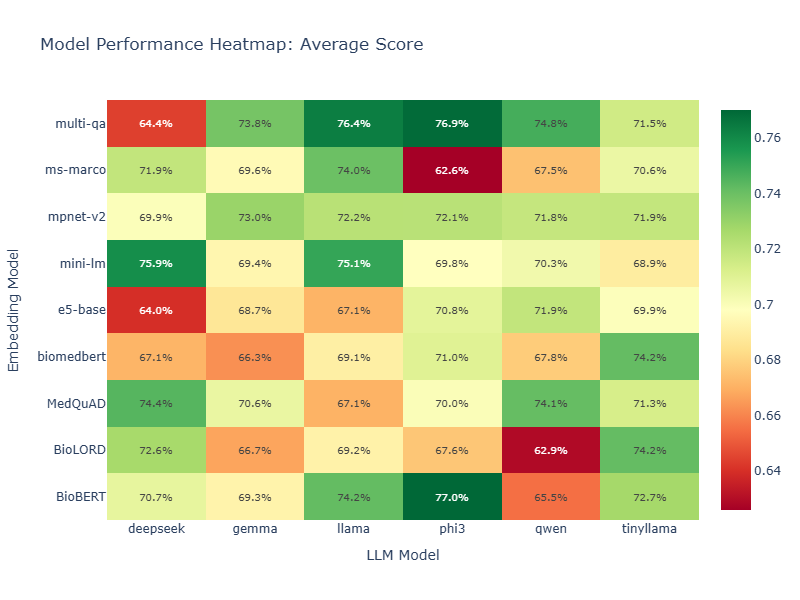
\includegraphics[width=\textwidth]{chap4_results/images/heatmap_average_score.png}
  \caption{Model comparison heatmap by average score.}
  \label{fig:heatmap_avg_score}
\end{figure}

\section{Top-Performing Configurations}
Table~\ref{tab:top_configs} reports the top configurations by average score. We report pass rate and average search time to capture effectiveness and efficiency trade-offs.

\newcolumntype{P}[1]{>{\centering\arraybackslash}p{#1}}
\newcolumntype{Y}{>{\centering\arraybackslash}X}

\begin{table}[h]
\centering
\begin{footnotesize}
\renewcommand\arraystretch{0.95}
\begin{tabularx}{\textwidth}{l l P{1.6cm} P{1.6cm} P{1.8cm}}
  \toprule
  Embedding & LLM & Pass rate & Avg. score & Avg. search time (s) \\
  \midrule
  BioBERT & phi3 & 100\% & 0.770 & 67.70 \\
  multi-qa & llama & 95\% & 0.764 & 61.20 \\
  multi-qa & phi3 & 95\% & 0.769 & 70.77 \\
  mini-lm & deepseek & 95\% & 0.759 & 326.02 \\
  mini-lm & llama & 100\% & 0.751 & 56.50 \\
  MedQuAD & deepseek & 90\% & 0.744 & 355.67 \\
  BioBERT & llama & 90\% & 0.742 & 82.48 \\
  BioLORD & tinyllama & 95\% & 0.742 & 73.44 \\
  biomedbert & tinyllama & 95\% & 0.742 & 355.25 \\
  MedQuAD & qwen & 95\% & 0.741 & 69.12 \\
  \bottomrule
\end{tabularx}
\end{footnotesize}
\caption{Top-performing configurations by average score.}
\label{tab:top_configs}
\end{table}

\paragraph{Observations.} The best average scores are achieved by BioBERT + phi3 and multi-qa + phi3/llama. MiniLM pairs (mini-lm + llama/deepseek) are strong with excellent pass rates; however, mini-lm + deepseek exhibits much longer search time, suggesting backend or retrieval interaction overhead. MedQuAD-based embeddings produce competitive average scores but at times with slower end-to-end latency.

\section{Efficiency and Safety}
We summarize representative efficiency and safety outcomes in Table~\ref{tab:efficiency_safety}. Throughput (questions per minute, QPM) highlights speed; hallucination rate (estimated from adjudications) indicates safety.

\begin{table}[h]
\centering
\begin{footnotesize}
\renewcommand\arraystretch{0.95}
\begin{tabularx}{0.9\textwidth}{l l P{1.3cm} P{1.4cm} P{1.5cm}}
  \toprule
  Embedding & LLM & QPM & Avg. score & Hallucination \\
  \midrule
  e5-base & deepseek & 1.122 & 0.640 & 0.40 \\
  mini-lm & qwen & 1.100 & 0.703 & 0.30 \\
  mini-lm & llama & 1.059 & 0.751 & 0.15 \\
  MedQuAD & deepseek & 0.169 & 0.744 & 0.10 \\
  \bottomrule
\end{tabularx}
\label{tab:efficiency_safety}
  \bottomrule
\end{tabularx}
\end{footnotesize}
\caption{Efficiency and safety metrics.}
\label{tab:efficiency_safety}
\end{table}

\paragraph{Trade-offs.} The fastest pipeline (e5-base + deepseek) sacrifices some answer quality relative to the top-scoring setups. Mini-lm + llama offers an appealing balance: perfect pass rate, good average score, high throughput, and low hallucination. The safest configuration by hallucination rate (MedQuAD + deepseek) is slower; this may reflect conservative generation behavior or heavier retrieval.

\section{Discussion}
Overall, average score is a more discriminative primary KPI than pass rate, revealing nuanced differences among competitive pairs. Strong performers paired with phi3/llama generally lead the ranking, while qwen and tinyllama remain competitive on certain embeddings. Category analysis indicates substantial headroom for structured clinical facts (labs, microbiology, prescriptions); targeted retrieval improvements (e.g., table-aware chunking, ontology-linked indices) and instruction-tuned prompts for evidence citation are likely to close this gap. Finally, efficiency/safety analysis underscores practical deployment choices: mini-lm + llama emerges as a well-balanced default; BioBERT + phi3 is optimal for peak accuracy; and e5-base + deepseek can serve latency-sensitive workflows when moderate quality is acceptable.

\section*{Artifacts}
The following artifacts are available in the results folder for reproducibility and further analysis: heatmap PNG and interactive HTML, the consolidated CSVs (results\_dataframe.csv, per\_question\_results.csv), efficiency/safety metrics (run\_efficiency\_and\_safety.csv), and the summary report (summary\_report.md).

% -----------------------------------------
% Evaluation methodology and metric rationale
% -----------------------------------------
\section{Evaluation Methodology and Metrics}
This section explains each evaluation we report, why it matters for clinical RAG, and how to interpret it.

\subsection{Average Score (primary KPI)}
The average score is a normalized 0--1 rating aggregated across questions. It reflects overall answer quality by combining rubric criteria such as factual correctness, sufficiency of evidence, and clinical appropriateness. We prioritize this as the primary KPI because it is sensitive to partial improvements that pass/fail metrics may miss and aligns with qualitative judgments of clinical usefulness.

\subsection{Pass Rate}
Pass rate is the proportion of questions meeting a minimum threshold (``acceptable'' grade). It is intuitive and robust, enabling quick comparisons of reliability. However, it is coarse; it does not distinguish between barely passing and very strong answers, so we pair it with the average score.

\subsection{Factual Accuracy and Performance Subscores}
Where available, we report separate subscores (e.g., factual accuracy, performance/presentation). Factual accuracy captures grounding to retrieved evidence and correctness of clinical facts; performance captures clarity, organization, and adherence to instructions (e.g., concise rationale, citations). Separating these clarifies whether errors arise from retrieval grounding or from generation quality.

\subsection{Latency and Throughput}
Average search time (seconds) measures end-to-end latency per question, dominated by retrieval plus model generation. Throughput (questions per minute, QPM) summarises system capacity under load. Clinical settings often require timely responses; we therefore report both and examine speed/quality trade-offs (e.g., e5-base + deepseek is fastest but with lower average score than top-accuracy pairs).

\subsection{Retrieval Coverage}
Average documents found provides a coarse proxy for retrieval depth and coverage. Too few documents may under-support grounding; too many may add noise and increase latency. Configurations that maintain strong scores with modest document counts indicate efficient, focused retrieval.

\subsection{Safety Indicators}
Hallucination rate approximates the frequency of unsupported or factually incorrect statements. Lower is safer. Disclaimer rate captures frequency of safety/compliance disclaimers; in clinical RAG, some disclaimers are appropriate, but overuse can reduce usefulness. We interpret these together with quality metrics to identify safe and useful operating points.

\subsection{Per-Question Analysis}
Per-question results (in \texttt{per\_question\_results.csv}) enable drill-down into failure modes (e.g., missing lab values, incorrect medication dosages) and success cases. These analyses inform targeted improvements (schema-aware chunking, ontology-linked retrieval, citation prompting).

% A compact summary table for quick reference
\begin{table}[h]
\centering
\begin{footnotesize}
\renewcommand\arraystretch{0.95}
\begin{tabular}{l p{6.2cm} p{6.2cm}}
  \toprule
  Metric & What it measures & Why it matters in clinical RAG \\
  \midrule
  Average score & Overall answer quality (0--1) across questions & Sensitive to partial improvements; aligns with perceived clinical usefulness \\
  Pass rate & Fraction of answers meeting an acceptability threshold & Simple reliability signal; complements average score \\
  Factual accuracy & Grounding and correctness of clinical facts & Directly tied to patient safety and evidence use \\
  Performance/presentation & Structure, clarity, instruction adherence & Affects readability, clinician trust, and efficiency \\
  Search time & Latency per question (s) & Practical responsiveness for clinical workflows \\
  Throughput (QPM) & Questions processed per minute & Capacity planning and cost/performance trade-offs \\
  Documents found & Retrieval depth/coverage proxy & Balances evidence sufficiency vs. noise/latency \\
  Hallucination rate & Unsupported/incorrect content frequency & Safety and risk mitigation \\
  Disclaimer rate & Frequency of safety disclaimers & Compliance vs. usefulness balance \\
  \bottomrule
\end{tabular}
\end{footnotesize}
\caption{Summary of evaluation metrics and their importance in clinical RAG.}
\label{tab:metrics_summary}
\end{table}

% Auto-generated comprehensive tables
\section{Comprehensive Tables}
To aid reproducibility, we include the full set of runs and category-wise averages generated from the consolidated CSVs.

\subsection{All 54 Runs (sorted by average score)}
% Note: Replace this with actual table content when available
\begin{center}
\begin{footnotesize}
\renewcommand\arraystretch{0.95}
% Auto-generated from results_dataframe.csv and run_efficiency_and_safety.csv
\begin{tabularx}{\textwidth}{l l c c c c}
  \toprule
  Embedding & LLM & Pass rate (\%) & Avg. score & Search time (s) & QPM \
  \midrule
  BioBERT & phi3 & 100.0 & 0.770 & 67.70 & 0.884 \
  multi-qa & phi3 & 95.0 & 0.769 & 70.77 & 0.845 \
  multi-qa & llama & 95.0 & 0.764 & 61.20 & 0.978 \
  mini-lm & deepseek & 95.0 & 0.759 & 326.02 & 0.184 \
  mini-lm & llama & 100.0 & 0.751 & 56.50 & 1.059 \
  multi-qa & qwen & 95.0 & 0.748 & 72.68 & 0.823 \
  MedQuAD & deepseek & 90.0 & 0.744 & 355.67 & 0.169 \
  biomedbert & tinyllama & 95.0 & 0.742 & 355.25 & 0.169 \
  BioLORD & tinyllama & 95.0 & 0.742 & 73.44 & 0.815 \
  BioBERT & llama & 90.0 & 0.742 & 82.48 & 0.725 \
  MedQuAD & qwen & 95.0 & 0.741 & 69.12 & 0.865 \
  ms-marco & llama & 90.0 & 0.740 & 72.60 & 0.822 \
  multi-qa & gemma & 90.0 & 0.738 & 77.55 & 0.772 \
  mpnet-v2 & gemma & 100.0 & 0.730 & 74.35 & 0.805 \
  BioBERT & tinyllama & 95.0 & 0.727 & 69.87 & 0.856 \
  BioLORD & deepseek & 90.0 & 0.726 & 65.96 & 0.907 \
  mpnet-v2 & llama & 85.0 & 0.722 & 69.29 & 0.863 \
  mpnet-v2 & phi3 & 90.0 & 0.721 & 61.62 & 0.971 \
  e5-base & qwen & 100.0 & 0.719 & 66.99 & 0.893 \
  ms-marco & deepseek & 95.0 & 0.719 & 71.14 & 0.841 \
  mpnet-v2 & tinyllama & 95.0 & 0.719 & 79.34 & 0.754 \
  mpnet-v2 & qwen & 100.0 & 0.718 & 65.52 & 0.913 \
  multi-qa & tinyllama & 85.0 & 0.715 & 70.61 & 0.847 \
  MedQuAD & tinyllama & 90.0 & 0.713 & 67.55 & 0.885 \
  biomedbert & phi3 & 90.0 & 0.710 & 69.87 & 0.856 \
  e5-base & phi3 & 100.0 & 0.708 & 60.60 & 0.986 \
  BioBERT & deepseek & 90.0 & 0.707 & 69.83 & 0.857 \
  MedQuAD & gemma & 85.0 & 0.706 & 70.92 & 0.843 \
  ms-marco & tinyllama & 80.0 & 0.706 & 62.50 & 0.957 \
  mini-lm & qwen & 90.0 & 0.703 & 54.39 & 1.100 \
  MedQuAD & phi3 & 90.0 & 0.700 & 68.14 & 0.878 \
  e5-base & tinyllama & 95.0 & 0.699 & 353.18 & 0.170 \
  mpnet-v2 & deepseek & 90.0 & 0.699 & 67.78 & 0.883 \
  mini-lm & phi3 & 85.0 & 0.698 & 353.36 & 0.170 \
  ms-marco & gemma & 90.0 & 0.696 & 61.34 & 0.975 \
  mini-lm & gemma & 100.0 & 0.694 & 61.13 & 0.979 \
  BioBERT & gemma & 95.0 & 0.693 & 67.09 & 0.892 \
  BioLORD & llama & 90.0 & 0.692 & 70.04 & 0.854 \
  biomedbert & llama & 85.0 & 0.691 & 71.43 & 0.838 \
  mini-lm & tinyllama & 90.0 & 0.689 & 67.78 & 0.883 \
  e5-base & gemma & 90.0 & 0.687 & 65.57 & 0.912 \
  biomedbert & qwen & 80.0 & 0.678 & 58.61 & 1.020 \
  BioLORD & phi3 & 85.0 & 0.676 & 69.92 & 0.856 \
  ms-marco & qwen & 85.0 & 0.675 & 66.41 & 0.901 \
  e5-base & llama & 85.0 & 0.671 & 63.97 & 0.935 \
  biomedbert & deepseek & 80.0 & 0.671 & 359.51 & 0.167 \
  MedQuAD & llama & 80.0 & 0.671 & 63.43 & 0.943 \
  BioLORD & gemma & 85.0 & 0.667 & 66.66 & 0.897 \
  biomedbert & gemma & 85.0 & 0.663 & 69.77 & 0.858 \
  BioBERT & qwen & 80.0 & 0.655 & 62.70 & 0.954 \
  multi-qa & deepseek & 75.0 & 0.644 & 70.20 & 0.852 \
  e5-base & deepseek & 80.0 & 0.640 & 53.28 & 1.122 \
  BioLORD & qwen & 75.0 & 0.629 & 66.17 & 0.904 \
  ms-marco & phi3 & 80.0 & 0.626 & 64.61 & 0.926 \
  \bottomrule
\end{tabularx}
\end{footnotesize}
\end{center}


\section{Additional Figures}
\begin{figure}[h]
  \centering
  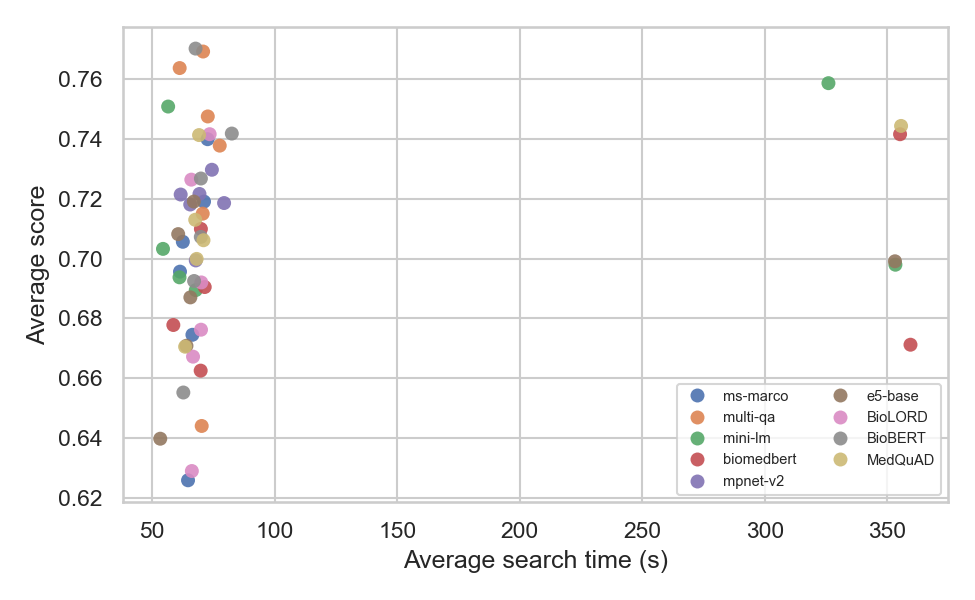
\includegraphics[width=\textwidth]{chap4_results/images/time_vs_score.png}
  \caption{Average score vs. average search time across all runs. Lower time and higher score are better.}
  \label{fig:time_vs_score}
\end{figure}

\begin{figure}[h]
  \centering
  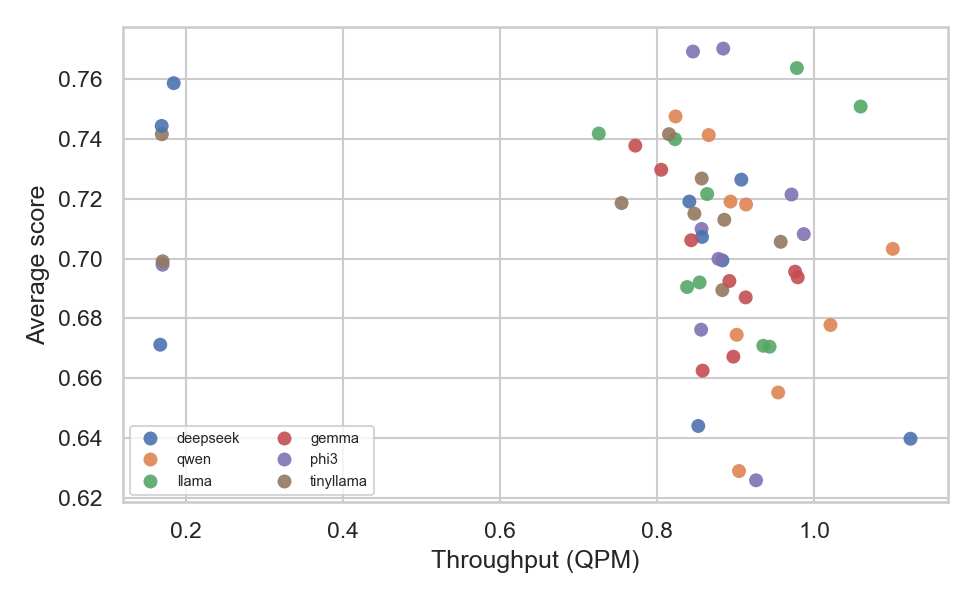
\includegraphics[width=\textwidth]{chap4_results/images/quality_vs_throughput.png}
  \caption{Average score vs. throughput (QPM). Useful to identify speed-quality efficient frontiers.}
  \label{fig:quality_vs_throughput}
\end{figure}

\begin{figure}[h]
  \centering
  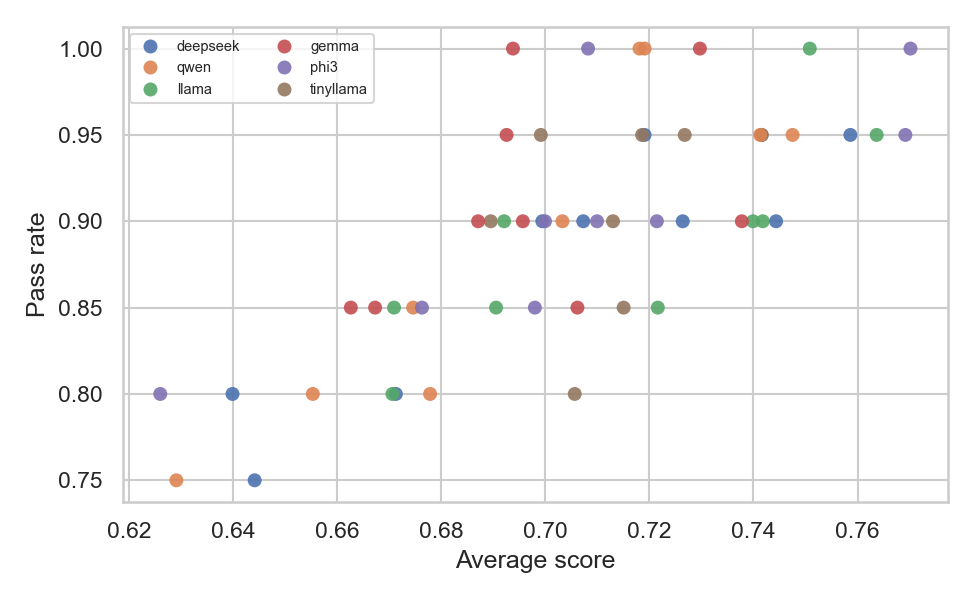
\includegraphics[width=\textwidth]{chap4_results/images/pass_rate_vs_score.png}
  \caption{Pass rate vs. average score by LLM. Highlights pairs that both pass reliably and score highly.}
  \label{fig:pass_rate_vs_score}
\end{figure}